\documentclass[11pt]{article}
%Created on 4/10/07.
\usepackage{enumerate}
\usepackage[OT1]{fontenc}
\usepackage{amsmath,amssymb}
\usepackage{natbib}
\usepackage[usenames]{color}
%\usepackage[dvips]{graphicx}
%\usepackage{bm}

\usepackage{smile}
\usepackage{natbib}
\usepackage{multirow}
\usepackage{listings}
% \usepackage{geometry}
\usepackage{pdflscape}
\usepackage{rotating}
\usepackage{todonotes}
%\usepackage{subfigure}
%\usepackage{makecell}
\usepackage[colorlinks = false,
            % linkcolor=red,
            % anchorcolor=blue,
            % citecolor=blue
            ]{hyperref}
            
\def\reals{{\mathbb R}}
\def\P{{\mathbb P}}
\def\E{{\mathbb E}}
\def\B{{\mathbb B}}
\def\htheta{\widehat \btheta}
\def\ttheta{\widetilde \btheta}
\def\hSigma{\w
idehat \bSigma}
\def\hS{\widehat S}
\def\hR{\widehat \Rb}
\def\hu{\widehat \bu}
\def\hK{\hat \Kb}
\def\beps{\bm{\epsilon}}

\def\argmin{\mathop{\text{\rm arg\,min}}}
\def\argmax{\mathop{\text{\rm arg\,max}}}
\def\given{{\,|\,}}
\def\ds{\displaystyle}
\def\bs{\backslash}
\def\R{{\mathcal{R}}}
\def\sign{\mathrm{sign}}

\def\card{\mathop{\text{card}}}
\def\rank{\mathrm{rank}}
\def\skeptic{{\sc skeptic}}
\def\NPN{\mbox{\it NPN}}
\def\vec{\mathop{\text{vec}}}
\def\tr{\mathrm{Tr}}
\def\trc{\mathop{\text{TRC}}}

\newcommand*{\Sc}{\cS^{\perp}}
\newcommand*{\Ac}{\cA^{\perp}}
\newcommand*{\supp}{\mathrm{supp}}

\newcommand{\cGS}{\mathcal{GS}}

\allowdisplaybreaks

\def\given{\,|\,}
\def\biggiven{\,\big{|}\,}
\def\tr{\mathop{\text{tr}}\kern.2ex}
\def\tZ{{\tilde Z}}
\def\tX{{\tilde X}}
\def\tR{{\tilde r}}
\def\tU{{\tilde U}}
\def\P{{\mathbb P}}
\def\E{{\mathbb E}}
\def\B{{\mathbb B}}

\def\sign{\mathop{\text{sign}}}
\def\supp{\mathop{\text{supp}}}
\def\card{\mathop{\text{card}}}
\def\rank{\mathrm{rank}}
\long\def\comment#1{}
\def\skeptic{{\sc skeptic}}
\def\NPN{\bPiox{\it NPN}}
\def\vec{\mathop{\text{vec}}}
\def\tr{\mathop{\text{Tr}}}
\def\trc{\mathop{\text{TRC}}}
\def\cS{{\mathcal{S}}}
\def\dr{\displaystyle \rm}
\def\skeptic{{\sc skeptic}}
\providecommand{\bnorm}[1]{\Big\vvvert#1\Big\vvvert}
\providecommand{\norm}[1]{\vvvert#1\vvvert}

\newcommand{\bel}{\begin{eqnarray}\label}
\newcommand{\eel}{\end{eqnarray}}
\newcommand{\bes}{\begin{eqnarray*}}
\newcommand{\ees}{\end{eqnarray*}}
\def\bess{\bes\small }
\def\Shat{{\widehat S}}
\def\lam{\rho}
\def\real{{\mathbb{R}}}
\def\R{{\real}}
\def\Ti{T_{\rm init}}
\def\Tm{T_{\rm main}}
\def\bcdot{{\bm \cdot}}
\newcommand{\red}{\color{red}}
\newcommand{\blue}{\color{blue}}
\newcommand{\la}{\langle}
\newcommand{\ra}{\rangle}
\newcommand{\cIs}{\cI_{\hat{s}}}

\let\oldemptyset\emptyset
\let\emptyset\varnothing

\newcommand{\op}{o_{\raisemath{-1.5pt}\PP}}
\newcommand{\Op}{O_{\raisemath{-1.5pt}\PP}}

\usepackage{mathrsfs}

\usepackage{fullpage}
\renewcommand{\baselinestretch}{1.0}

\def\sep{\;\big|\;}
\newcommand{\chz}[1]{{\textcolor{red}{[CHZ: #1]}}}
\newcommand{\hf}[1]{{\textcolor{red}{[FH: #1]}}}
\def \trunc{\mathop{\text{trunc}}}
\def \obs {{\rm obs}}
\def \mis {{\rm mis}}
\def \hbSigma {\widehat{\bSigma}}
\def \bbSigma {\bar{\bSigma}}

\usepackage{hyperref}
%\usepackage[protrusion=false,expansion=true]{microtype}
%\usepackage[activate={true,nocompatibility},final,tracking=true,kerning=true,spacing=true,factor=1100,stretch=10,shrink=10]{microtype}
\usepackage[    protrusion=true,
            expansion=true,
            final,
            babel
                ]{microtype}
\usepackage{setspace}
\usepackage{enumitem}
% \usepackage{parskip}
\lstset{frame=tb,
  language=Python,
  aboveskip=3mm,
  belowskip=3mm,
  showstringspaces=false,
  columns=flexible,
  basicstyle={\small\ttfamily},
  numbers=none,
  numberstyle=\tiny\color{gray},
  keywordstyle=\color{blue},
  commentstyle=\color{dkgreen},
  stringstyle=\color{mauve},
  breaklines=true,
  breakatwhitespace=true
  tabsize=3
}

%% Thesis requirements for binding
\usepackage[top=1in, bottom=1in, left=1.5in, right=1in]{geometry}
\usepackage{titling}


\begin{document}
\begin{titlepage}

\newcommand{\HRule}{\rule{.8\linewidth}{0.5mm}} % Defines a new command for the horizontal lines, change thickness here
\renewenvironment{abstract}
 {\small
  \begin{center}
  \bfseries \abstractname\vspace{-.5em}\vspace{0pt}
  \end{center}
  \list{}{
    \setlength{\leftmargin}{.5cm}%
    \setlength{\rightmargin}{\leftmargin}%
  }%
  \item\relax}
 {\endlist}


\center % Center everything on the page

%----------------------------------------------------------------------------------------
%   HEADING SECTIONS
%----------------------------------------------------------------------------------------

\textsc{\LARGE Princeton University}\\[0.5cm] % Name of your university/college
\textsc{\large Operations Research and Financial Engineering}\\[0.5cm] % Major heading such as course name

\vspace{2em}
%----------------------------------------------------------------------------------------
%   TITLE SECTION
%----------------------------------------------------------------------------------------

\HRule \\[0.2cm]
{ \LARGE \bfseries Applying Nested Statistical Models\\
for Temporal Affordance Learning\\
in Vision-Based Autonomous Driving\par} % Title of your document
\HRule \\[1.5cm]
 
\vspace{2em}
%----------------------------------------------------------------------------------------
%   AUTHOR SECTION
%----------------------------------------------------------------------------------------

\begin{minipage}{0.4\textwidth}
\begin{flushleft} \large
\emph{Author:}\\
Eddie \textsc{Zhou} % Your name
\end{flushleft}
\end{minipage}
~
\begin{minipage}{0.4\textwidth}
\begin{flushright} \large
\emph{Advisor:} \\
Professor Han \textsc{Liu} % Supervisor's Name
\end{flushright}
\end{minipage}\\[1cm]

\vspace{2em}
%----------------------------------------------------------------------------------------
%   LOGO SECTION
%----------------------------------------------------------------------------------------
\begin{figure}[H]
\centering

\includegraphics[width=30mm]{figs/princeton_shield}
\end{figure}

\vspace{4em}
 
%----------------------------------------------------------------------------------------
\textsc{
Submitted in partial fulfillment\\
of the requirements for the degree of\\
Bachelor of Science in Engineering\\
Department of Operations Research and Financial Engineering\\
Princeton University
}\\[0.5cm]

\vspace{2em}
%----------------------------------------------------------------------------------------
%   DATE SECTION
%----------------------------------------------------------------------------------------

\textsc{\large April 2016}\\[5mm] % Date, change the \today to a set date if you want to be precise
\pagestyle{empty}

%----------------------------------------------------------------------------------------
% Statements
%----------------------------------------------------------------------------------------

\begin{minipage}{\textwidth}
\begin{flushleft} \large
\textsc{I hereby declare that I am the sole author of this thesis.}\par
\vspace{1em}
\textsc{I authorize Princeton University to lend this thesis to other institutions or individuals for
the purpose of scholarly research.}
\vspace{6em}
\end{flushleft}
\begin{flushright}
\noindent\begin{tabular}{ll}
\makebox[2.5in]{\hrulefill}{\hrulefill}\\
\textsc{Eddie Zhou}\\
\end{tabular}
\end{flushright}
\vspace{6em}
\begin{flushleft} \large
\textsc{I further authorize Princeton University to reproduce this thesis by photocopying or by
other means, in total or in part, at the request of other institutions or individuals for the
purpose of scholarly research.}
\vspace{6em}
\end{flushleft}
\begin{flushright}
\noindent\begin{tabular}{ll}
\makebox[2.5in]{\hrulefill}{\hrulefill}\\
\textsc{Eddie Zhou}\\
\end{tabular}
\end{flushright}
\end{minipage}

\pagestyle{empty}
\newpage
%----------------------------------------------------------------------------------------
% Acknowledgements
%----------------------------------------------------------------------------------------
\begin{minipage}{\textwidth}
{ \LARGE \bfseries Acknowledgements\par}
\parskip=\baselineskip \advance\parskip by 0pt plus 2pt
First, I would like to thank my advisor, Professor Han Liu.  He has been an amazing teacher and constant guiding hand as an advisor.  His dedication to furthering the fields of statistics and machine learning has inspired my academic and professional pursuits.  He has also helped me understand the importance of brevity alongside statistical parsimony, and is the reason you are reading 16 and not 66 pages.  Additionally, I would like to thank Chenyi Chen, the original DeepDriver, for answering my countless questions about this project and others.

I would also like to thank my family.  To Mom and Dad -- you have both set inspiring examples for how to live your lives as students, professionals, and people.  I am eternally grateful for your work in building the springboard that launched my collegiate and professional life.  Steve -- it's immeasurably easier to walk a road paved by someone else, and I am forever indebted to you for that.

To all my friends at Princeton -- I thank each and every one of you for bringing out a different side of me, and helping me understand myself and grow.  Wollack, Katz, Dingus, Ploppy, Daway, Eric, Bee and many others -- you've helped define this place for me.

Finally, to Sarah -- we did it.  Here's to the next chapter.
\end{minipage}

\end{titlepage}
\chapter{Part 1}
\title{\huge Nested Statistical Models for Temporal Affordance Learning in Vision-Based Autonomous Driving}
\author{
Eddie Zhou\thanks{Department of Operations Research and Financial Engineering, Princeton University, Princeton, NJ 08544, USA; e-mail: {\tt edzhou@princeton.edu}},~~
Chenyi Chen\thanks{Department of Operations Research and Financial Engineering, Princeton University, Princeton, NJ 08544, USA; e-mail: {\tt chenyi@princeton.edu}},~~
Han Liu\thanks{Department of Operations Research and Financial Engineering, Princeton University, Princeton, NJ 08544,USA; e-mail: {\tt hanliu@princeton.edu}}, ~ and
Alain Kornhauser\thanks{Department of Operations Research and Financial Engineering, Princeton University, Princeton, NJ 08544, USA; e-mail: {\tt alaink@princeton.edu}}
}
\date{}
\maketitle
% \vspace{-1em}
\begin{abstract}
Most current autonomous vehicle systems largely rely on LIDAR, but there is much room for development in vision-based systems.  Recently, a DeepDriving paradigm of learning affordance indicators from input images was suggested.  We extend this model by analyzing the temporal and sequential nature of the input images.  To do so, we apply convolutional feature extraction and examining three problems: the usefulness of history, the lag selection problem, and the viability of complex models with history.  We train recurrent, or ``nested'' statistical models of varying complexity, and our results demonstrate that the sequential aspect of this problem is highly important and appropriate for recurrent statistical models.
\end{abstract}
\vspace{1em}
\noindent {\bf Keywords:} convolutional neural network; nested models; recurrent; autonomous driving; image recognition, regression, multivariate adaptive regressive splines.
\section{Introduction}\label{intro}
Predictive statistical models are formulated, trained, and used in a variety of applications, from spam filtering and recommender systems to outlier detection and image recognition.  One such application that has not been thoroughly explored from a statistical standpoint is autonomous driving.  Within this application, vision-based approaches typically adopt one of two paradigms: mediated perception (parsing an entire scene to make a driving decision), and behavior reflex (mapping an input image to a driving action).  \cite{deepdriving} proposed an intermediate, ``DeepDriving'' paradigm that struck a balance between the two: in their work, image representations are mapped onto a small set of affordance indicator values (distances to lane markings, angles, etc.).  These values are then passed to a simple logic controller that operates the vehicle accordingly.\par
DeepDriving still relies on a model that maps an input vector $\mathbf{x} \in \mathbb{R}^n$ and outputs a vector of continuous values $\mathbf{y} \in \mathbb{R}^m$, which points to the task of statistical regression.  While the problem of image classification is largely solved with the advancement of deep learning methods (namely, deep convolutional neural networks), our image regression problem is slightly different.  The more important aspect of the data at hand is its temporal and sequential nature -- in a real setting, images captured by the autonomous vehicle would be processed one after another, and at a realistic granularity, previous images should affect the current driving decisions.  \cite{deepdriving} relied largely on the widely-used convolutional neural networks to map input images to the aforementioned affordance indicator.  While powerful, convnets do not take advantage of any temporal features in the data, as recurrent neural networks do.\par
Our goal for this paper, however, is not simply to replace their work with convolutional neural networks, which contain a recurrency.  We look to apply rigorous statistical analysis to investigate the role of history in predicting affordance indicator values, and subsequently understand the viability of this history in both linear and nonlinear models.  We characterize our approach in three problems: the first is to rigorously determine whether past history is predictively useful at all.  To do so, we build simple linear models and use p-value analysis for the relevant coefficients.  Second, we look to solve the lag order selection problem, which tells us exactly how much history is useful, doing so through model selection using modified evaluation metrics.  Finally, we examine the predictive viability of nonlinear models operating on historical, lag order selected data, hoping to show that the usefulness of history extends to more complex models.\par
\subsection{Related Works}
This paper largely builds off of \cite{deepdriving}'s work in validating the DeepDriving or direct perception paradigm.  As mentioned in Section \ref{intro}, they train a convolutional neural network with data extracted from the TORCS driving video game.  The inputs are convoluted image features, while the output is a set of 14 continuous values: the affordance indicators passed to the logic controller.  The output data is available via extraction from the game engine, as are the input images (which are passed through a convnet for feature extraction).  Note that in our work, we also use the dataset presented in their work.  Doing so allows us to investigate the temporal nature within the same assumptions and exact same dataset.\par
We also make use of work done by \cite{aic_bic1}, \cite{aic_bic2}, and \cite{liew} in the usage of model selection metrics with respect to the lag order selection problem.  The convolutional neural network used in our work also relies on the standard structure set forth by \cite{lenet}.  Our nonlinear work is advanced by the seminal paper on MARS, by \cite{mars}, as well as the fast heuristic added in \cite{fastmars}.
\subsection{Paper Organization}
The rest of this paper is organized as follows. Section \ref{sec:data_tools} introduces details of the dataset, explains the feature extraction process, and gives a brief summary of the software used for model fitting.  In Sections \ref{sec:single_history}, \ref{sec:lag_order}, \ref{sec:nonlinear}, we refine the three problems presented: whether history is predictively valuable, rigorously determining the lag order, and examining the viability of more complex, nonlinear models.  Section \ref{sec:results} provides numerical and graphical results for the three problems, and section \ref{sec:discussion} contains discussion thereof.  All code is available for examination and reproduction in a \href{https://github.com/edz504/thesis}{Github repository} located at \url{https://github.com/edz504/thesis} (see \lstinline{project1}).
\newpage
\section{Data Wrangling and Tools}\label{sec:data_tools}
\subsection{Data Pipeline}
The TORCS dataset exists as a leveldb, so we use Python's \lstinline{leveldb} module to connect and read from it. We also need to use Python's Caffe interface to access the Datum objects stored -- iterating through the leveldb, we fill \lstinline{numpy} arrays of dimension 10000 x 3 x 210 x 280, and use \lstinline{hickle} to dump the batched arrays. The dimensions are explained as follows: the data is 3 color channels, each image is of resolution 210 x 280, and 10000 is the largest even data size that fits in memory. We also extract the 14 affordance indicators (true values) for each of the 484815 images and store the resulting matrix separately.
\subsection{Feature Extraction}
We first trained a convolutional neural network with LeNet architecture as first proposed by \cite{lenet} for the purpose of feature extraction.  We implement the network with \lstinline{nolearn} combined with \lstinline{Lasagne} and \lstinline{Theano} -- each response variable is scaled to [0, 1] with the following:
\begin{align*}
y_{ij}^{(s)} = \frac{y_{ij} - \min_jy_{ij}}{\max_jy_{ij} - \min_jy_{ij}}
\end{align*}
during this process in order to facilitate convergence.  Data is loaded and subsequently passed through the model in the aforementioned batches of 10000.  We extract the features as the last hidden layer, which has 500 nodes.  Therefore, our final training matrix $\bX^{(CNN)}$ is 484815 x 500.
\subsection{Training and Testing}
In Section \ref{sec:single_history}, we use the Ordinary Least Squares implementation of the \lstinline{statsmodels} package in Python for our model training and evaluation.  Then, due to an increased need for computational efficiency, in \ref{sec:lag_order} and part of \ref{sec:nonlinear}, we use the \lstinline{scikit-learn} Python library for Stochastic Gradient Descent.  Finally, for one of our nonlinear models in \ref{sec:nonlinear} we use \lstinline{py-earth} for Multivariate Adaptive Regression Splines.
\section{Single History Inclusion}\label{sec:single_history}
We perform ordinary least squares regression with two model structures: one with the time $t$ convoluted image features as input, and one with both the time $t$ and time $t - 1$ convoluted image features as input.  For both ``Model 1'' and ``Model 2'' structures (indicated by $\hat{\mathbf{y}}_t$ and $\tilde{\mathbf{y}}_t$ respectively), we train 14 separate models, each predicting a single affordance indicator, or response variable.  The two models can be expressed in least squares regression modelling as the following:
\begin{align*}
\hat{\mathbf{y}}_t^{(a_1)} &= \bm{\beta}^{(a_1)}\mathbf{X_t} + \bm{\epsilon}\\
\tilde{\mathbf{y}}_t^{(a_1)} &= \bm{\beta_t}^{(a_1)}\mathbf{X_t} + \bm{\beta_{t-1}}^{(a_1)}\mathbf{X_{t-1}} + \bm{\epsilon}\\
\hat{\mathbf{y}}_t^{(a_2)} &= \bm{\beta}^{(a_2)}\mathbf{X_t} + \bm{\epsilon}\\
\tilde{\mathbf{y}}_t^{(a_2)} &= \bm{\beta_t}^{(a_2)}\mathbf{X_t} + \bm{\beta_{t-1}}^{(a_2)}\mathbf{X_{t-1}} + \bm{\epsilon}\\
&.\\&.\\&.\\
\hat{\mathbf{y}}_t^{(a_{14})} &= \bm{\beta}^{(a_{14})}\mathbf{X_t} + \bm{\epsilon}\\
\tilde{\mathbf{y}}_t^{(a_{14})} &= \bm{\beta_t}^{(a_{14})}\mathbf{X_t} + \bm{\beta_{t-1}}^{(a_{14})}\mathbf{X_{t-1}} + \bm{\epsilon}\\
\end{align*}
After fitting these 28 models with OLS, we will analyze the p-values for each coefficient, across all affordance indicators (500 x 14 for model 1, and 1000 x 14 for model 2).  As a brief reminder on the elementary statistics of least-squares coefficients, each coefficient's p-value is the result of a $t$-test with the null hypothesis that the coefficient itself is zero.  Therefore, finding significantly low values for the p-values corresponding to the coefficients of the past time step will demonstrate that history has predictive value within this model.
\section{Lag Order Selection}\label{sec:lag_order}
After we validate the significance of past history, the next step is to decide exactly how much history is relevant -- in other words, to examine the lag order selection problem.  To do this, we again fit a series of simple linear models -- however, each now corresponds to including varying amounts of history, from only the most recent image to the previous 12 images.  We wrangle the 484815 x 500 \textbf{X} matrix into 12 more matrices, each corresponding to using one more previous time step.  These are of dimension 484814 x 1000, 484813 x 1500, ... (note that we lose one more data point from the beginning of the temporal sequence with each time inclusion).\par
Naive OLS matrix inversion is no longer computationally viable for these larger matrices, so we use stochastic gradient descent with squared loss and an L2 penalty (ridge).  Due to the high dimensionality, we also use a high penalty multiplier to push parameters closer to 0, as well as a higher number of epochs in the stochastic gradient descent iterations.\par
For each model structure, and for each affordance indicator, two models are trained.  One is trained with all of the available data, and the other with 80\%, setting aside 20\% for testing.  Using the full-dataset-trained models, for each time inclusion limit $s$ (the number of time steps to include), we calculate both the Akaike and Bayesian ``stacked information criterion''.  These are versions of the standard AIC and BIC metrics that aggregate across each affordance indicator -- the time inclusion can be seen as a model ``structure'', so we want to compare these metrics for each time inclusion, not across the response variables.  Standard and stacked IC formulas are structured as follows:
\begin{align*}
&\text{AIC}(\boldsymbol\beta) = 2k - 2\log(\hat{L})\\
&\text{BIC}(\boldsymbol\beta) = k\log N - 2\log(\hat{L})\\
&\text{AIC}^{(t-s)}(\boldsymbol\beta^{(t-0)}, \boldsymbol\beta^{(t-1)}, ..., \boldsymbol\beta^{(t-s)}) = 2\sum_{a=1}^{14}k_a - 2\sum_{a=1}^{14}\log(\hat{L}_a)\\
&\text{BIC}^{(t-s)}(\boldsymbol\beta^{(t-0)}, \boldsymbol\beta^{(t-1)}, ..., \boldsymbol\beta^{(t-s)}) = \sum_{a=1}^{14}k_a\log N_a - 2\sum_{a=1}^{14}\log(\hat{L}_a)
\end{align*}
where $k$ is the model degree of freedom (number of non-zero predictor coefficients), and the log-likelihood is calculated as follows:
\begin{align*}
\log(\hat{L}) &= -\frac{N}{2}\log(2\pi\hat{\sigma}^2) - \frac{SSR}{2\hat{\sigma}^2}\\
SSR &= \sum_{i=1}^N(y_i - \hat{y}_i)\\
\hat{\sigma}^2 &= \frac{SSR}{N}
\end{align*}
We also use the 80\%-trained models to calculate RMSE on the remaining 20\% as test data.  This value can similarly be aggregated across all 14 affordance indicators for each time step, simply by summing all of the squared errors and $N$ values.
\begin{align*}
&RMSE(\boldsymbol\beta) = \sqrt{\frac{\sum_{i=1}^N(y_i - \hat{y}_i)}{N}}\\
&RMSE^{(t-s)}(\boldsymbol\beta^{(t-0)}, \boldsymbol\beta^{(t-1)}, ..., \boldsymbol\beta^{(t-s)}) = \sqrt{\frac{\sum_{a=1}^{14}\sum_{i=1}^N(y_{i, a} - \hat{y}_{i, a})}{\sum_{a=1}^{14}N_a}}
\end{align*}
\section{Nonlinear Models}\label{sec:nonlinear}
If we solve the lag order selection problem, we would like to examine if including history proves for predictive power beyond simple linear models.  We therefore choose to examine two nonlinear models with our selected lag order, and evaluate them on the prediction metrics given above to analyze their viability.
\subsection{Basis Expansion}
The first nonlinear model we explore is a simple basis expansion model.  There is an abundance of basis expansions that are viable, with infinite polynomial operations.  Because we are not concerned with feature-feature interaction and we wish to retain computational feasibility, however, we simply add a polynomial basis expansion for each response variable up to the third power.
\begin{align*}
\mathbf{x} &= [x_1, x_2, ..., x_k]\\
\mathbf{x}^{(expand)} &= [x_1, x_1^2, x_1^3, x_2, x_2^2, x_2^3, ..., x_k, x_k^2, x_k^3]
\end{align*}
Depending on the selected lag order $s$, the data will then have a new dimension of $1500s$, as each additional lag order provides another 500 dimensions, and the basis expansion provides another factor of 3.  After expanding the basis, it becomes a matter of fitting another simple linear model with stochastic gradient descent to the new, expanded data and evaluating it with an RMSE metric.\par
\subsection{Multivariate Adaptive Regressive Splines}
The next nonlinear framework to explore is multivariate adaptive regressive splines, introduced by \cite{mars}.  This process is a more complex nonlinear method than simply extending the basis and fitting a linear model.  As a non-parametric regression, MARS models non-linearities through basis functions composed of a constant, a hinge function, or a product of multiple hinge functions.  MARS training is done with a greedy forward pass that adds basis functions that give maximal reduction in SSR, followed by a backwards pass that prunes the model using generalized cross validation, which can be seen as a form of regularization.\par
Due to the expensive nature of the continual forward and backward passes, there are various heuristics to speed up the model.  The first heuristic proposed by the original author in \cite{fastmars} limits the maximum number of parents terms considered at each step of the forward pass.  It does so by cutting off the priority queue ranking of parent functions at some parameter $K$.\par
This fast heuristic is usually available in the implementations of MARS, and is controlled by varying the \lstinline{fast_K} parameter.  In general, lower values of the parameter decrease the training time (decreasing the number of parent terms considered), but at the expense of the quality of the model.  Higher values are generally supposed to take longer, but result in stronger models, but random variation makes this rule general rather than rigid, as per \cite{earth}.\par
\section{Results}\label{sec:results}
\subsection{History Inclusion}
The first model is simply predicting the response values as a linear function of the current time step's image features.  As expected, we see low p-values for a significant number of the 500 features.  For almost every affordance indicator, the median p-value (across all 500 coefficients) is less than 0.05, demonstrating that over half of the convoluted image features are significant in each of the 14 individual models.  The following table shows the distributions of these 500 p-values in the form of summary statistics for each affordance indicator.
\begin{table}[H]
\centering
\caption{p-value summary for Model 1  $\bm{\beta}$ coefficients.}
\begin{tabular}{@{}lllllll@{}}
\toprule
    & Min.       & 1st Qu.   & Median    & Mean   & 3rd Qu. & Max.   \\ \midrule
a1  & 0          & 1.541e-31 & 1.142e-05 & 0.2229 & 0.6058  & 0.9716 \\
a2  & 0          & 1.697e-05 & 0.1004    & 0.2926 & 0.6946  & 0.9889 \\
a3  & 7.275e-218 & 1.569e-12 & 0.02273   & 0.294  & 0.7537  & 0.9964 \\
a4  & 0          & 4.727e-10 & 0.04213   & 0.2813 & 0.6944  & 0.9874 \\
a5  & 0          & 1.655e-14 & 0.009673  & 0.1359 & 0.1436  & 0.9978 \\
a6  & 0          & 2.698e-13 & 0.007431  & 0.2    & 0.3722  & 0.9859 \\
a7  & 0          & 3.849e-14 & 0.003059  & 0.1093 & 0.05035 & 0.9935 \\
a8  & 0          & 3.372e-09 & 0.001924  & 0.1226 & 0.07164 & 0.9831 \\
a9  & 0          & 1.47e-06  & 0.06613   & 0.2064 & 0.3358  & 0.9971 \\
a10 & 0          & 9.744e-09 & 0.01287   & 0.1966 & 0.415   & 0.9866 \\
a11 & 0          & 4.802e-09 & 0.007885  & 0.1157 & 0.07668 & 0.9934 \\
a12 & 0          & 1.234e-10 & 0.005826  & 0.1    & 0.03029 & 0.9981 \\
a13 & 6.051e-291 & 2.937e-09 & 0.0194    & 0.2836 & 0.7434  & 0.9874 \\
a14 & 0          & 2.422e-07 & 0.00165   & 0.1384 & 0.1424  & 0.9953 \\ \bottomrule
\end{tabular}
\end{table}
In the second model, we input both the 500 convoluted image features of the current time step, as well as the 500 convoluted image features of the previous time step, for a total of 1000 features.  In the below tables, we see that the p-value distribution for the 500 $\bm{\beta_t}$ coefficients is larger than the corresponding distribution of 500 p-values in Model 1.  This is intuitive, though, given the addition of 500 new features not included in Model 1 -- more features inherently means that a parsimonious model will regard fewer features as important.  Moreover, the p-values for the $\bm{\beta_{t-1}}$ coefficients are overwhelmingly significant, which answers our question of interest.  It is clear that the features from the previous time step are significant in predicting affordance indicators for the current time step -- we include a graphical representation of the distribution of the $\bm{\beta_{t-1}}$ p-values for further confirmation. 
\begin{table}[H]
\centering
\caption{p-value summary for Model 2 $\bm{\beta_t}$ coefficients.}
\begin{tabular}{@{}lllllll@{}}
\toprule
    & Min.       & 1st Qu.   & Median   & Mean   & 3rd Qu. & Max.   \\ \midrule
a1  & 1.868e-287 & 2.627e-09 & 0.02677  & 0.2161 & 0.4138  & 0.9925 \\
a2  & 3.211e-106 & 0.009934  & 0.3882   & 0.4276 & 0.862   & 0.9988 \\
a3  & 1.271e-74  & 0.0003873 & 0.226    & 0.396  & 0.9093  & 0.9999 \\
a4  & 8.369e-128 & 0.0004557 & 0.2257   & 0.3932 & 0.8869  & 1      \\
a5  & 1.361e-81  & 0.0003228 & 0.04829  & 0.1531 & 0.1317  & 0.9982 \\
a6  & 1.681e-85  & 5.213e-05 & 0.1444   & 0.1871 & 0.2097  & 0.9908 \\
a7  & 4.051e-105 & 8.328e-05 & 0.01527  & 0.1447 & 0.1641  & 1      \\
a8  & 1.943e-135 & 0.0001521 & 0.0088   & 0.1519 & 0.1899  & 0.9959 \\
a9  & 4.69e-78   & 0.009723  & 0.1822   & 0.2368 & 0.3035  & 0.9915 \\
a10 & 8.137e-100 & 0.001327  & 0.1711   & 0.2912 & 0.5374  & 0.9975 \\
a11 & 3.133e-100 & 0.0004654 & 0.009569 & 0.1409 & 0.1303  & 0.9973 \\
a12 & 1.215e-151 & 0.0001589 & 0.008946 & 0.1281 & 0.1532  & 0.9921 \\
a13 & 6.864e-72  & 0.00198   & 0.2783   & 0.3594 & 0.7223  & 0.9886 \\
a14 & 1.091e-116 & 0.0005832 & 0.00637  & 0.1561 & 0.2204  & 0.9986 \\ \bottomrule
\end{tabular}
\end{table}
\begin{table}[H]
\centering
\caption{p-value summary for Model 2 $\bm{\beta_{t-1}}$ coefficients.}
\begin{tabular}{@{}lllllll@{}}
\toprule
    & Min.       & 1st Qu.   & Median   & Mean   & 3rd Qu. & Max.   \\ \midrule
a1  & 0          & 4.004e-14 & 0.001513 & 0.1808 & 0.401   & 0.9868 \\
a2  & 0          & 3.374e-05 & 0.0695   & 0.2896 & 0.6123  & 0.9954 \\
a3  & 1.875e-123 & 6.232e-08 & 0.04029  & 0.292  & 0.6005  & 0.9992 \\
a4  & 2.921e-150 & 4.874e-07 & 0.05511  & 0.2675 & 0.5239  & 0.9988 \\
a5  & 2.609e-193 & 3.417e-08 & 0.03431  & 0.1649 & 0.2446  & 0.9952 \\
a6  & 3.009e-183 & 1.626e-07 & 0.03167  & 0.1852 & 0.2335  & 0.9921 \\
a7  & 4.245e-292 & 1.435e-08 & 0.006297 & 0.1501 & 0.1567  & 0.9934 \\
a8  & 0          & 1.514e-06 & 0.005839 & 0.1487 & 0.1798  & 0.9977 \\
a9  & 0          & 1.412e-05 & 0.05789  & 0.2005 & 0.2799  & 0.9996 \\
a10 & 5.842e-206 & 4.892e-05 & 0.06788  & 0.2259 & 0.4497  & 0.9921 \\
a11 & 2.047e-131 & 1.548e-05 & 0.01567  & 0.1896 & 0.2996  & 0.9976 \\
a12 & 6.702e-140 & 9.075e-06 & 0.009431 & 0.1585 & 0.1948  & 0.9923 \\
a13 & 3.324e-69  & 0.0001888 & 0.07977  & 0.2762 & 0.6316  & 0.9882 \\
a14 & 3.431e-107 & 0.0001382 & 0.02132  & 0.1873 & 0.2827  & 0.9939 \\ \bottomrule
\end{tabular}
\label{m2_t-1}
\end{table}
\begin{figure}[H]
\vspace{6em}
\centering
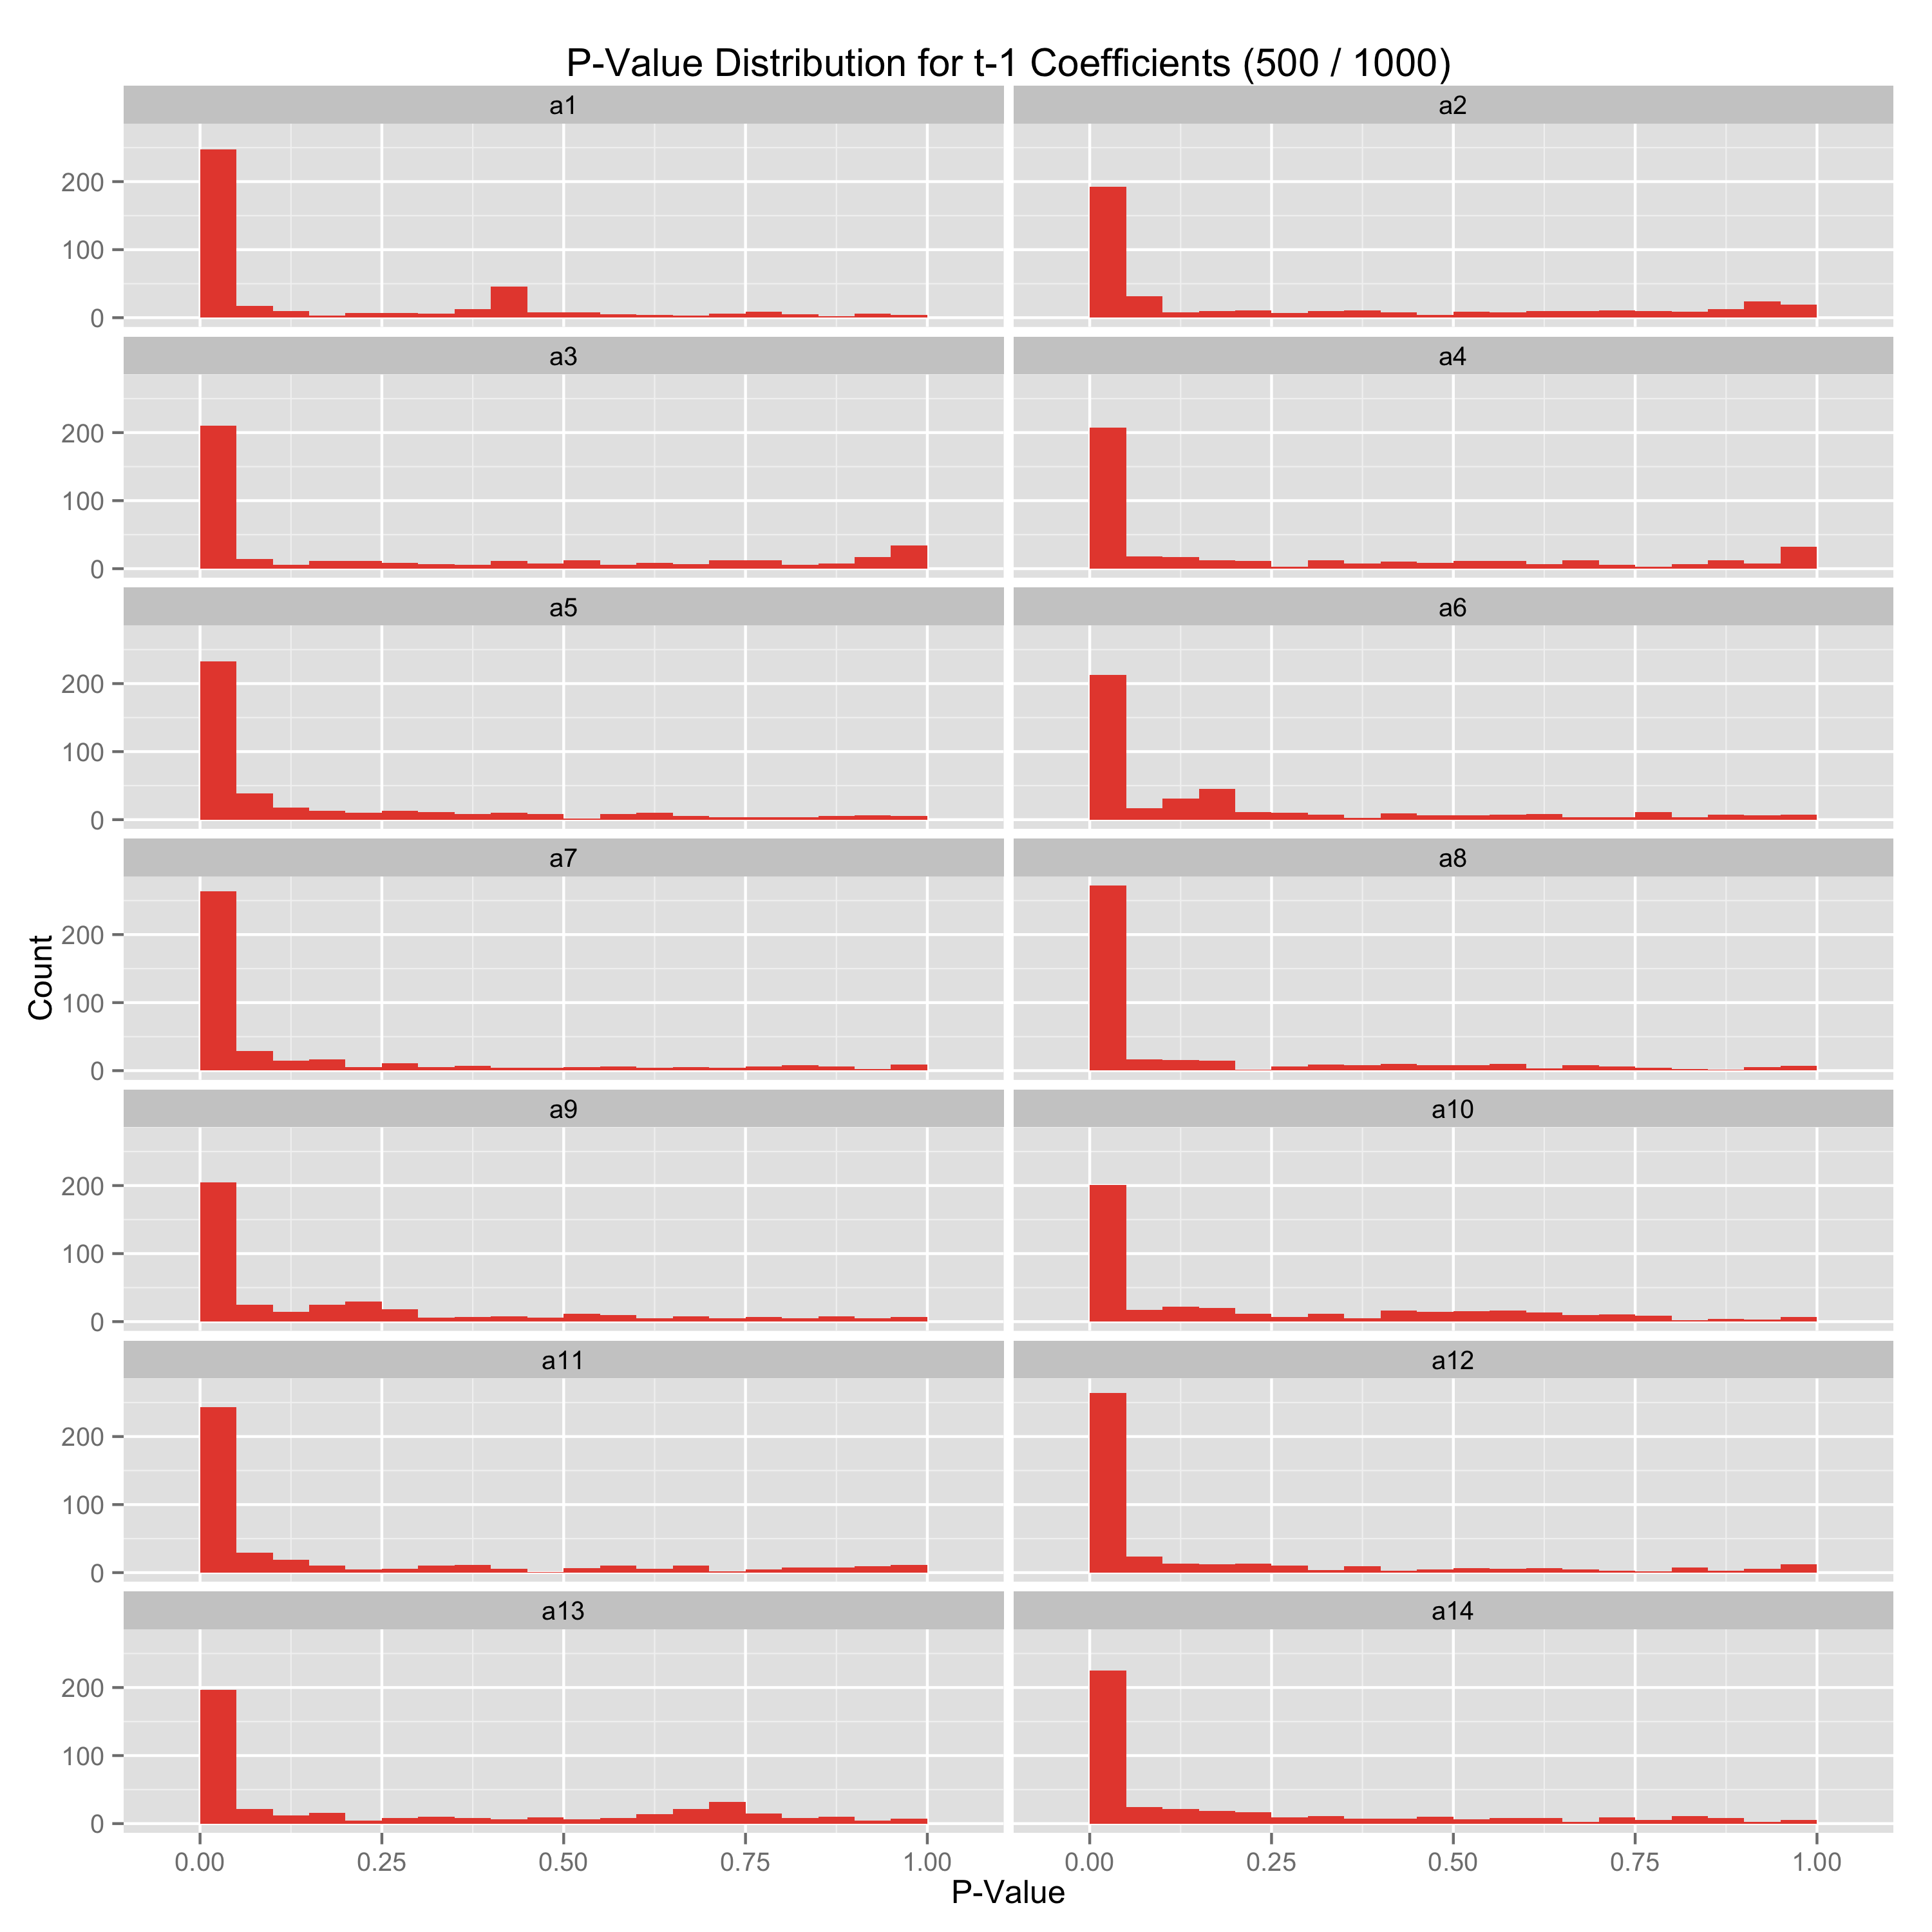
\includegraphics[width=155mm]{figs/t1_tminus1_pvals.png}
\caption{The distributions of the t-1 step p-values in Model 2 structure.}
\label{fig:p_dist}
\end{figure}
\newpage
\subsection{Lag Order Selection}\label{sec:lag-order-results}
As described in Section \ref{sec:lag_order}, we calculate stacked information criterion and aggregate RMSE values for each additional inclusion of history, plotting them with LOESS-smoothed lines below.
\begin{figure}[H]
\centering
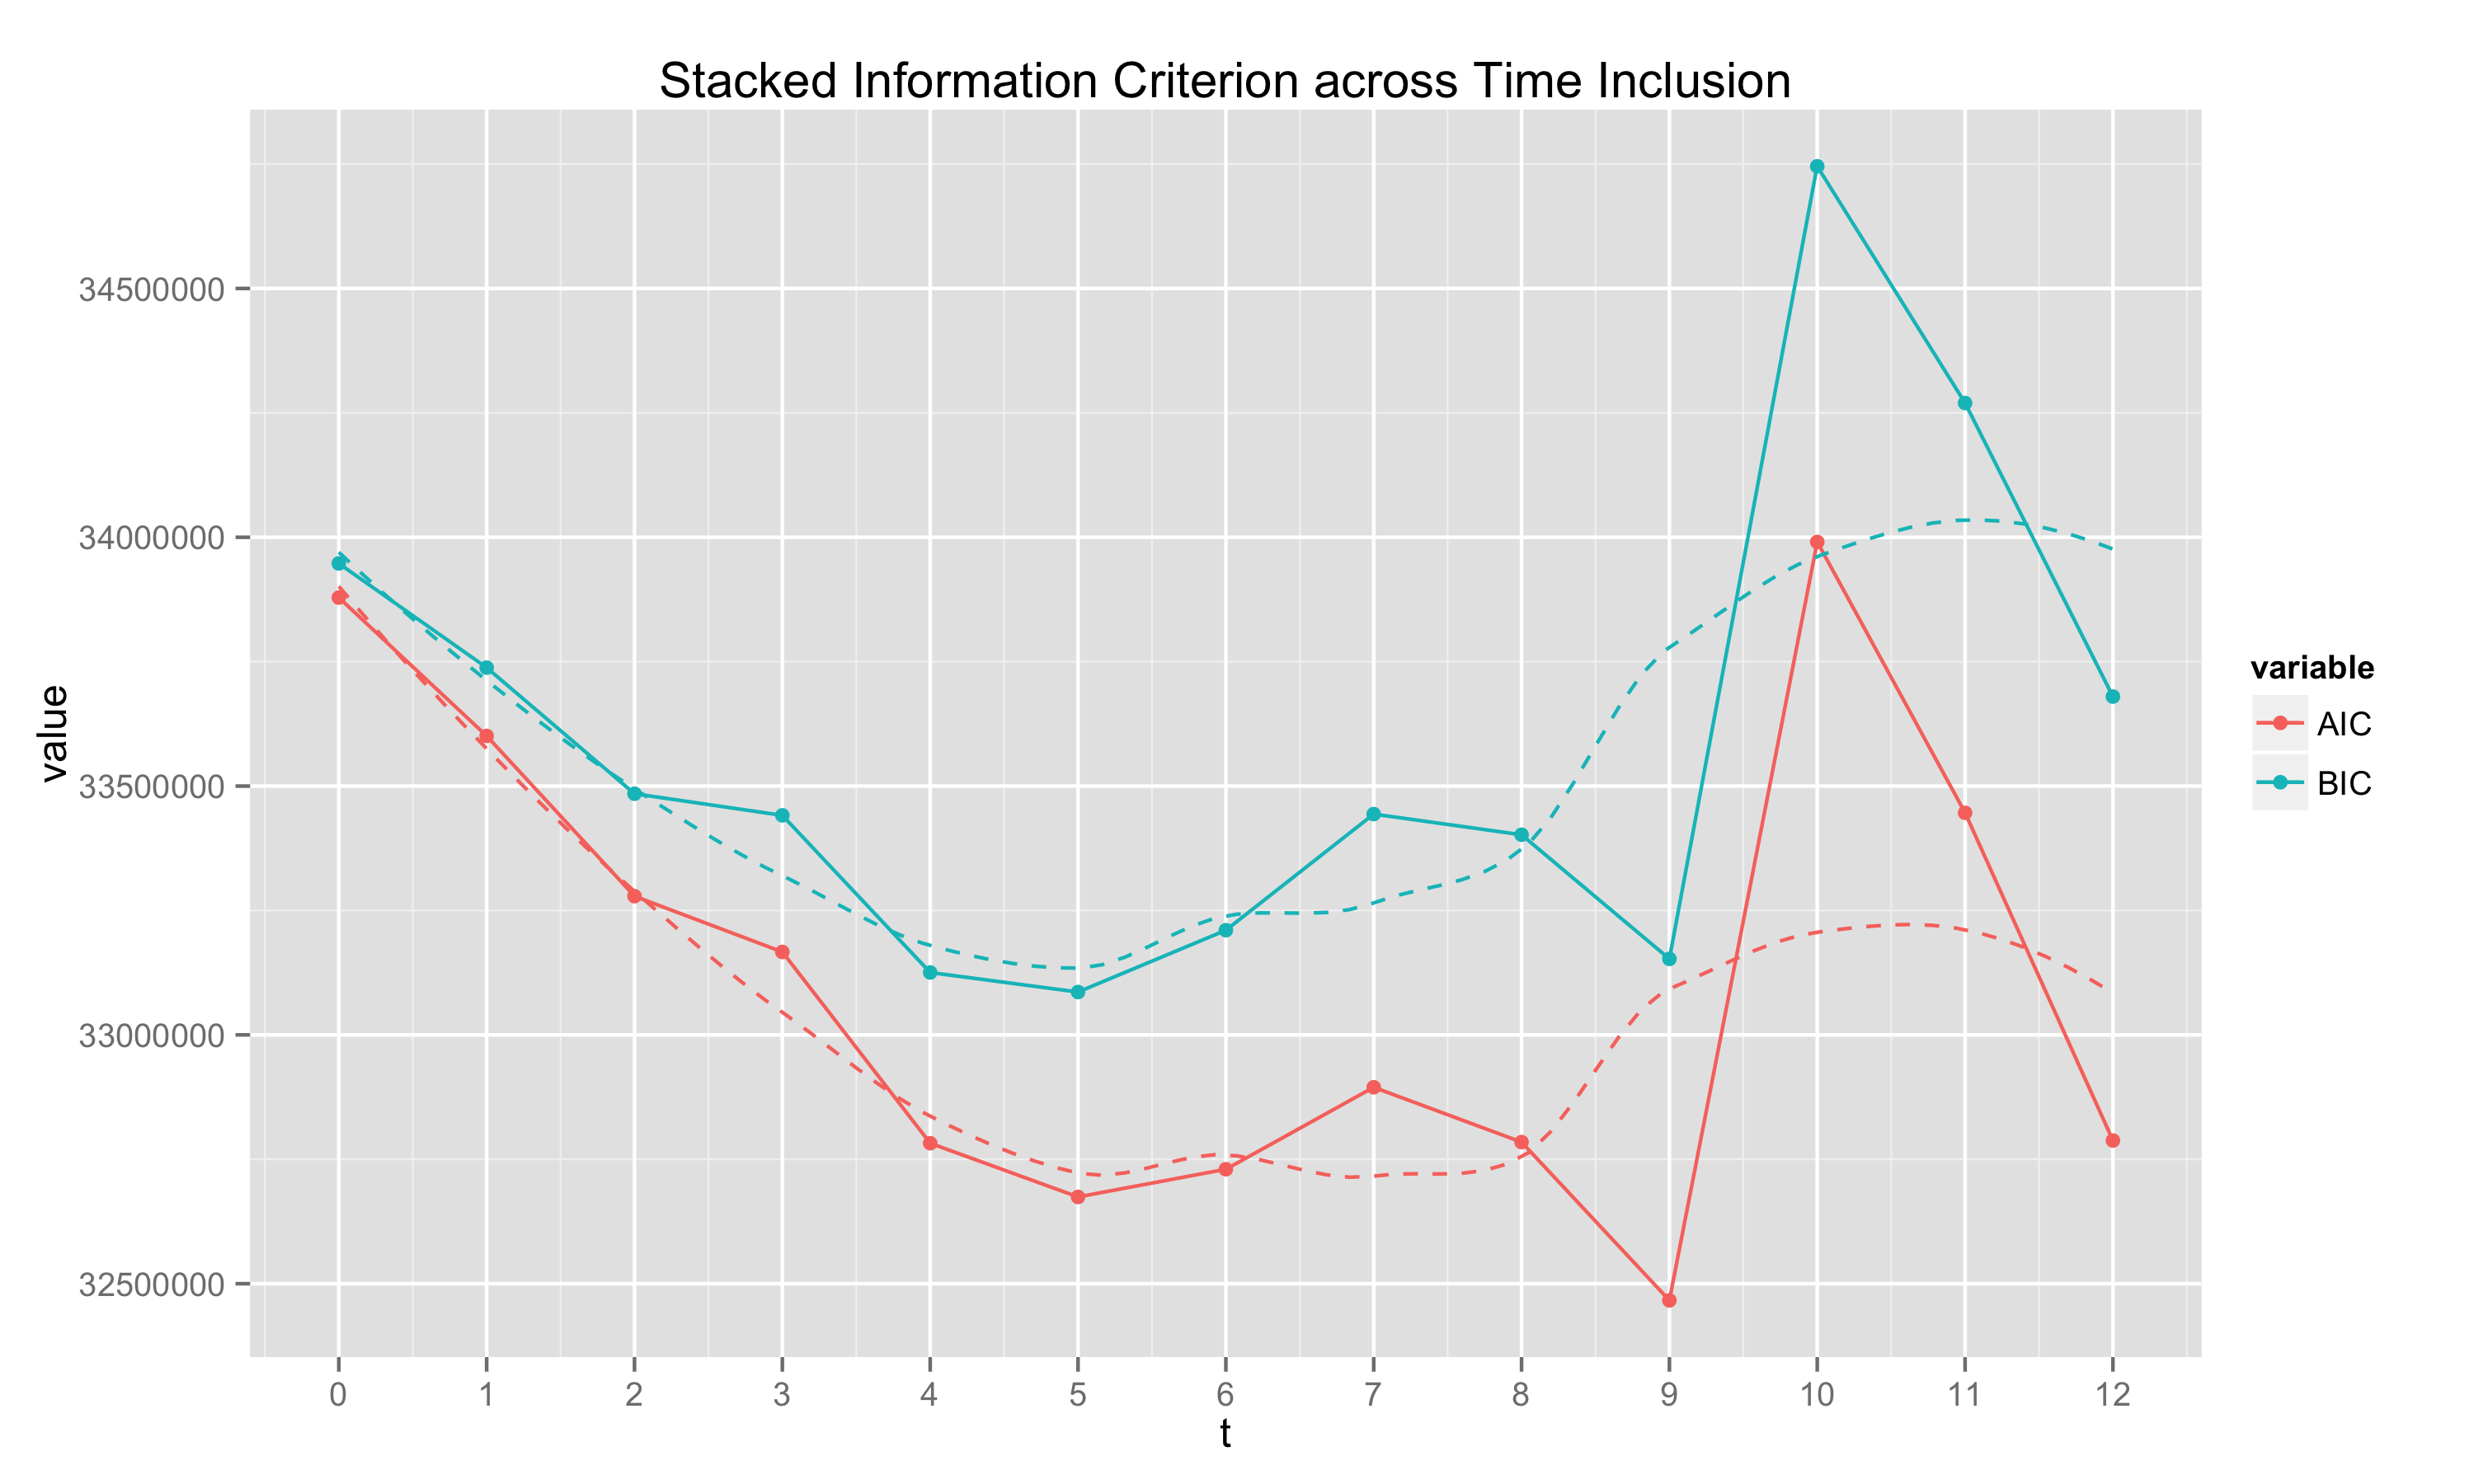
\includegraphics[width=160mm]{figs/sgd_stacked_ic.png}
% \caption{Stacked AIC and BIC}
\label{fig:stacked_ic}
\end{figure}
\begin{figure}[H]
\centering
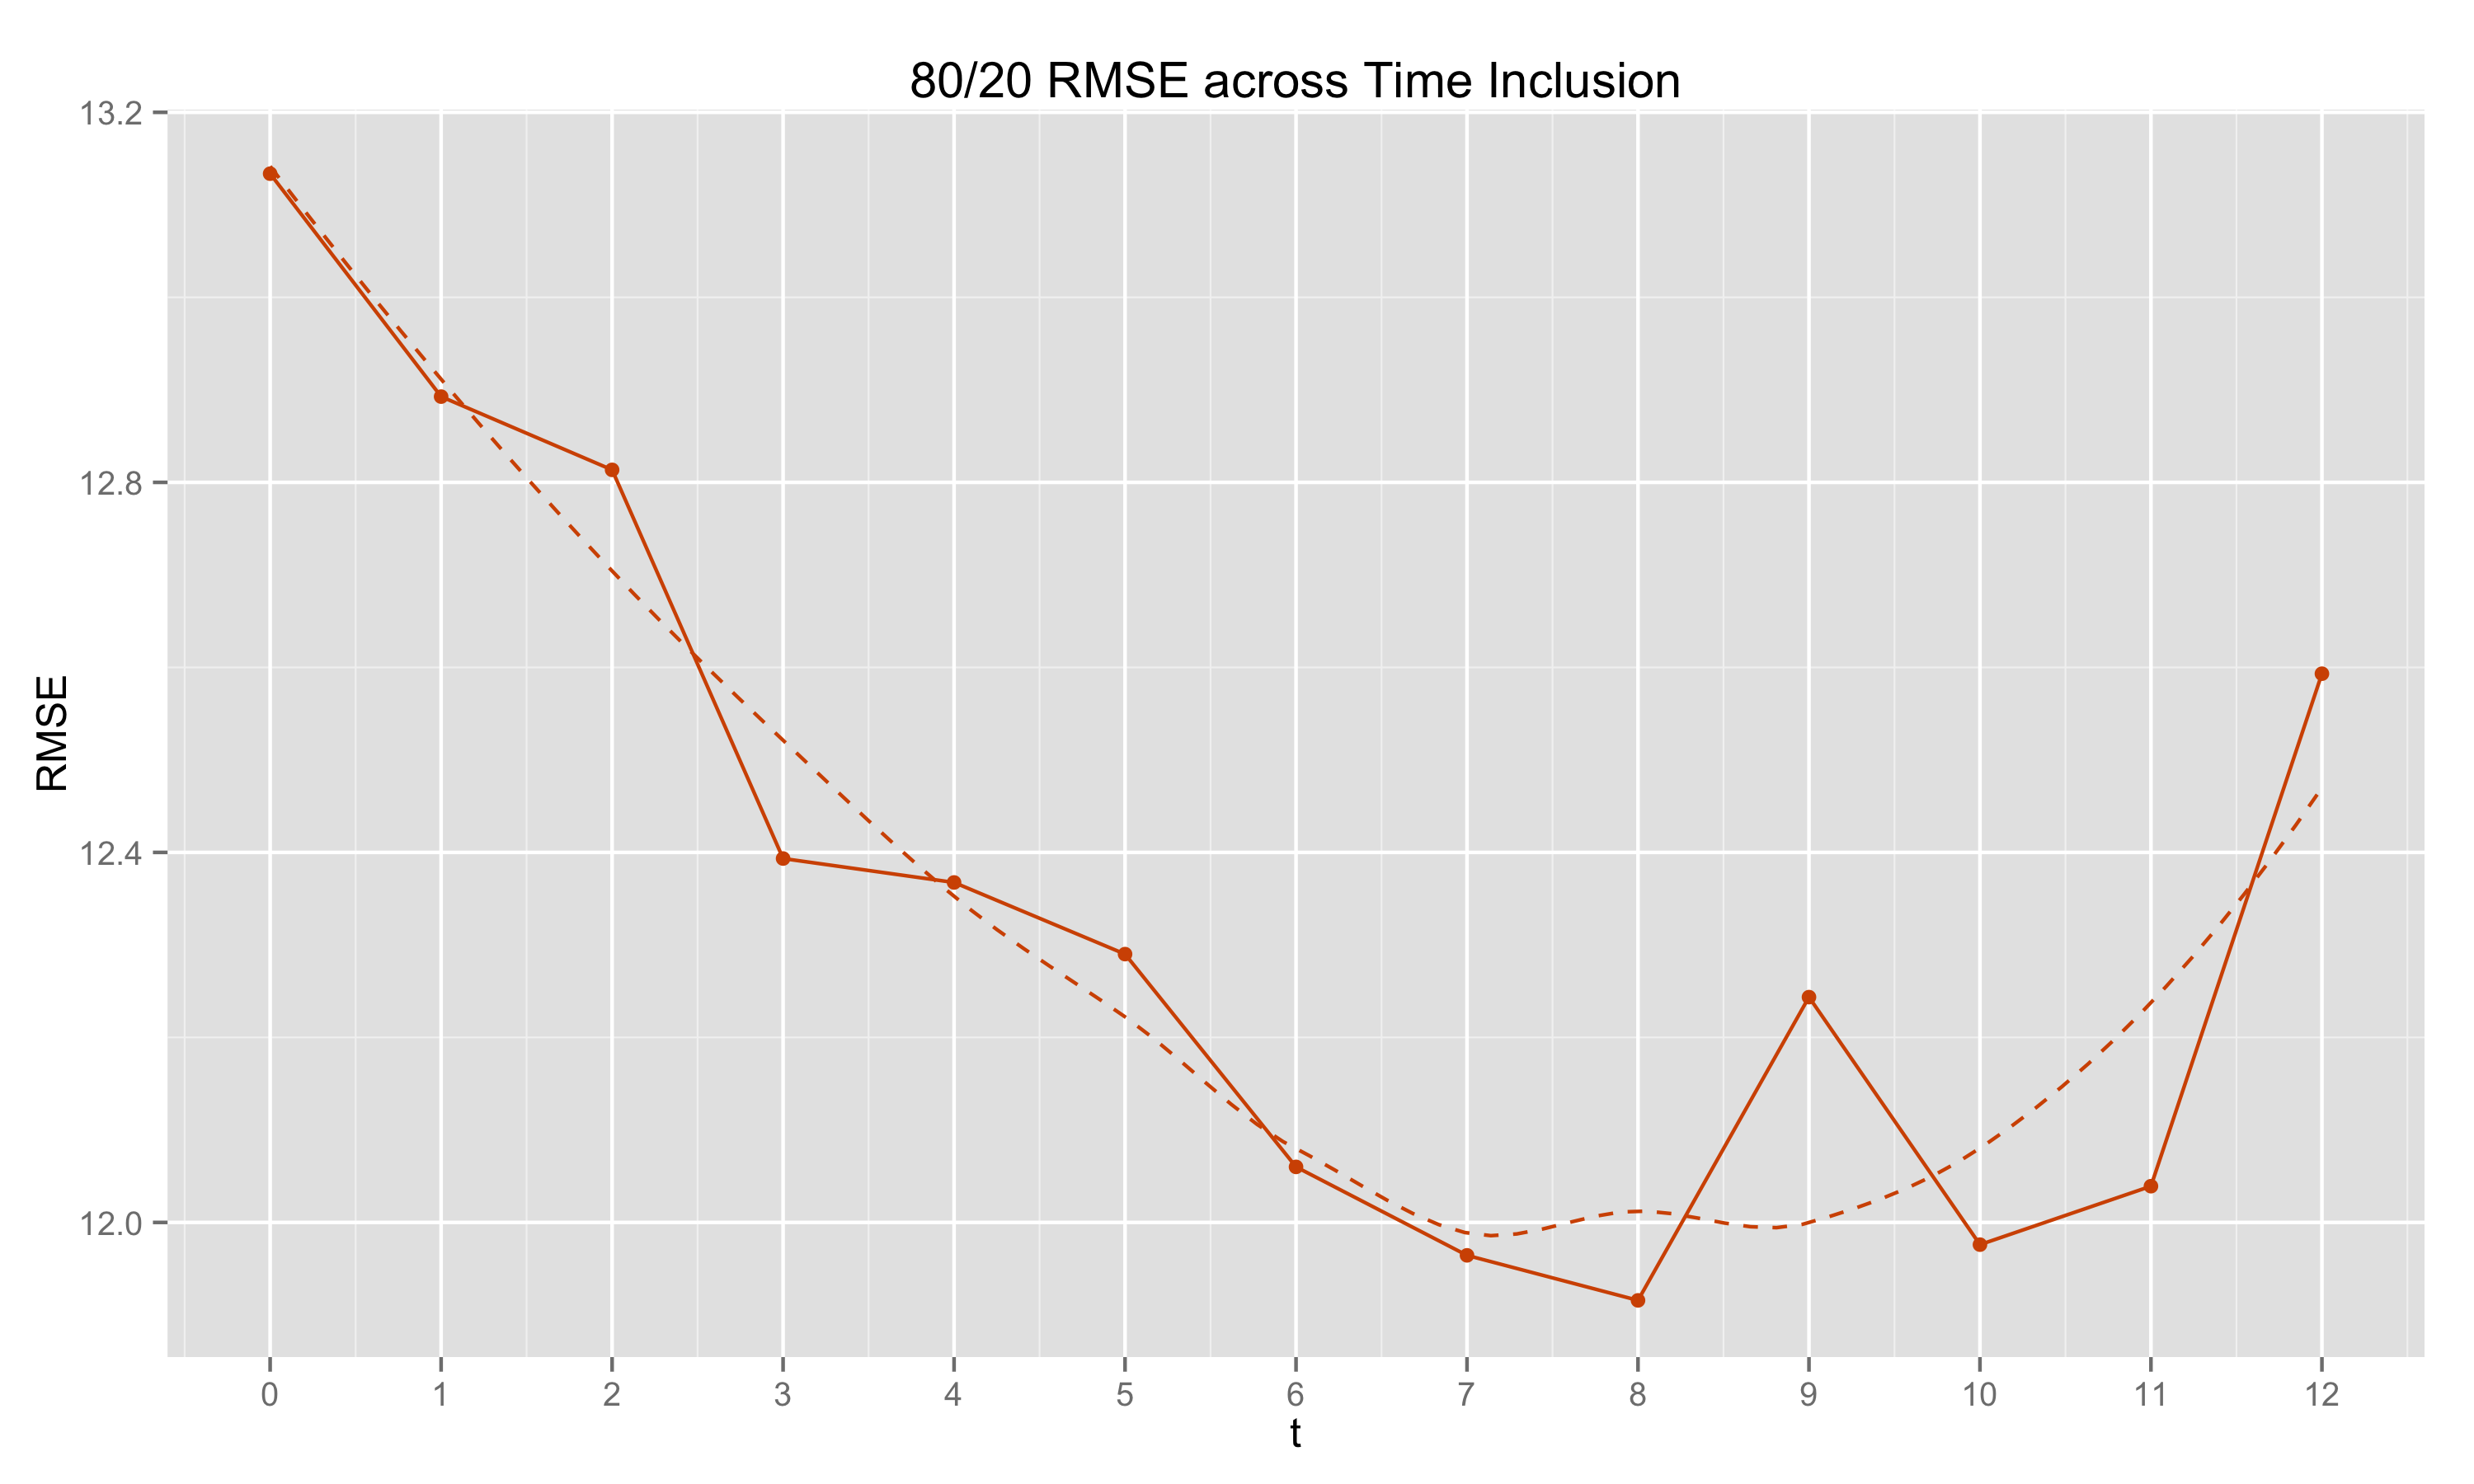
\includegraphics[width=150mm]{figs/sgd_rmse.png}
% \caption{Aggregated RMSE}
\label{fig:rmse}
\end{figure}
In the stacked information criterion plot, we see a steady decrease of both AIC and BIC as we include more history, until we get to $t-5$.  When we include the past 6 convoluted features, though, both of the information criterion begin to rise again, and we see much more noise.  In the aggregated RMSE plot, we see a similarly convex curve that decreases until around $t-7$, and then begins rising (again, with more noise on the ascent).  It is clear that there is a decrease, followed by a noisy increase, and that the smallest value lies somewhere in the aforementioned range.\par
The implementation of the stacked IC and the nature of RMSE dictates that smaller values point to better models.  In using these metrics, we note that BIC seeks the ``true'' model, whereas AIC tries to select the model that most adequately describes an unknown, high dimensional reality, as described by \cite{aic_bic1}, \cite{aic_bic2}.  Moreover, in the lag order selection literature, \cite{liew} showed that AIC exists as the best lag length selection criteria.  Low RMSE values also point directly to predictive power, so we move forward with the $t-7$ model structure pointed to by the LOESS-smoothed AIC and RMSE results.
\subsection{Nonlinear Models}
\subsubsection{Basis Expansion}
For our basis-expanded linear models, we train a variety of models, varying the hyperparameter $\alpha$, which controls regularization within stochastic gradient descent.  The below plot shows, however, this basis expansion does not result in a consistent decrease in RMSE over the $t-7$ linear model selected by the methodology of Section \ref{sec:lag_order}.  Different values of the regularization parameter $\alpha$ did not succeed in achieving lower RMSEs than the best simple linear models, which were below 12.0 (see Section \ref{sec:lag-order-results}).
\begin{figure}[H]
\centering
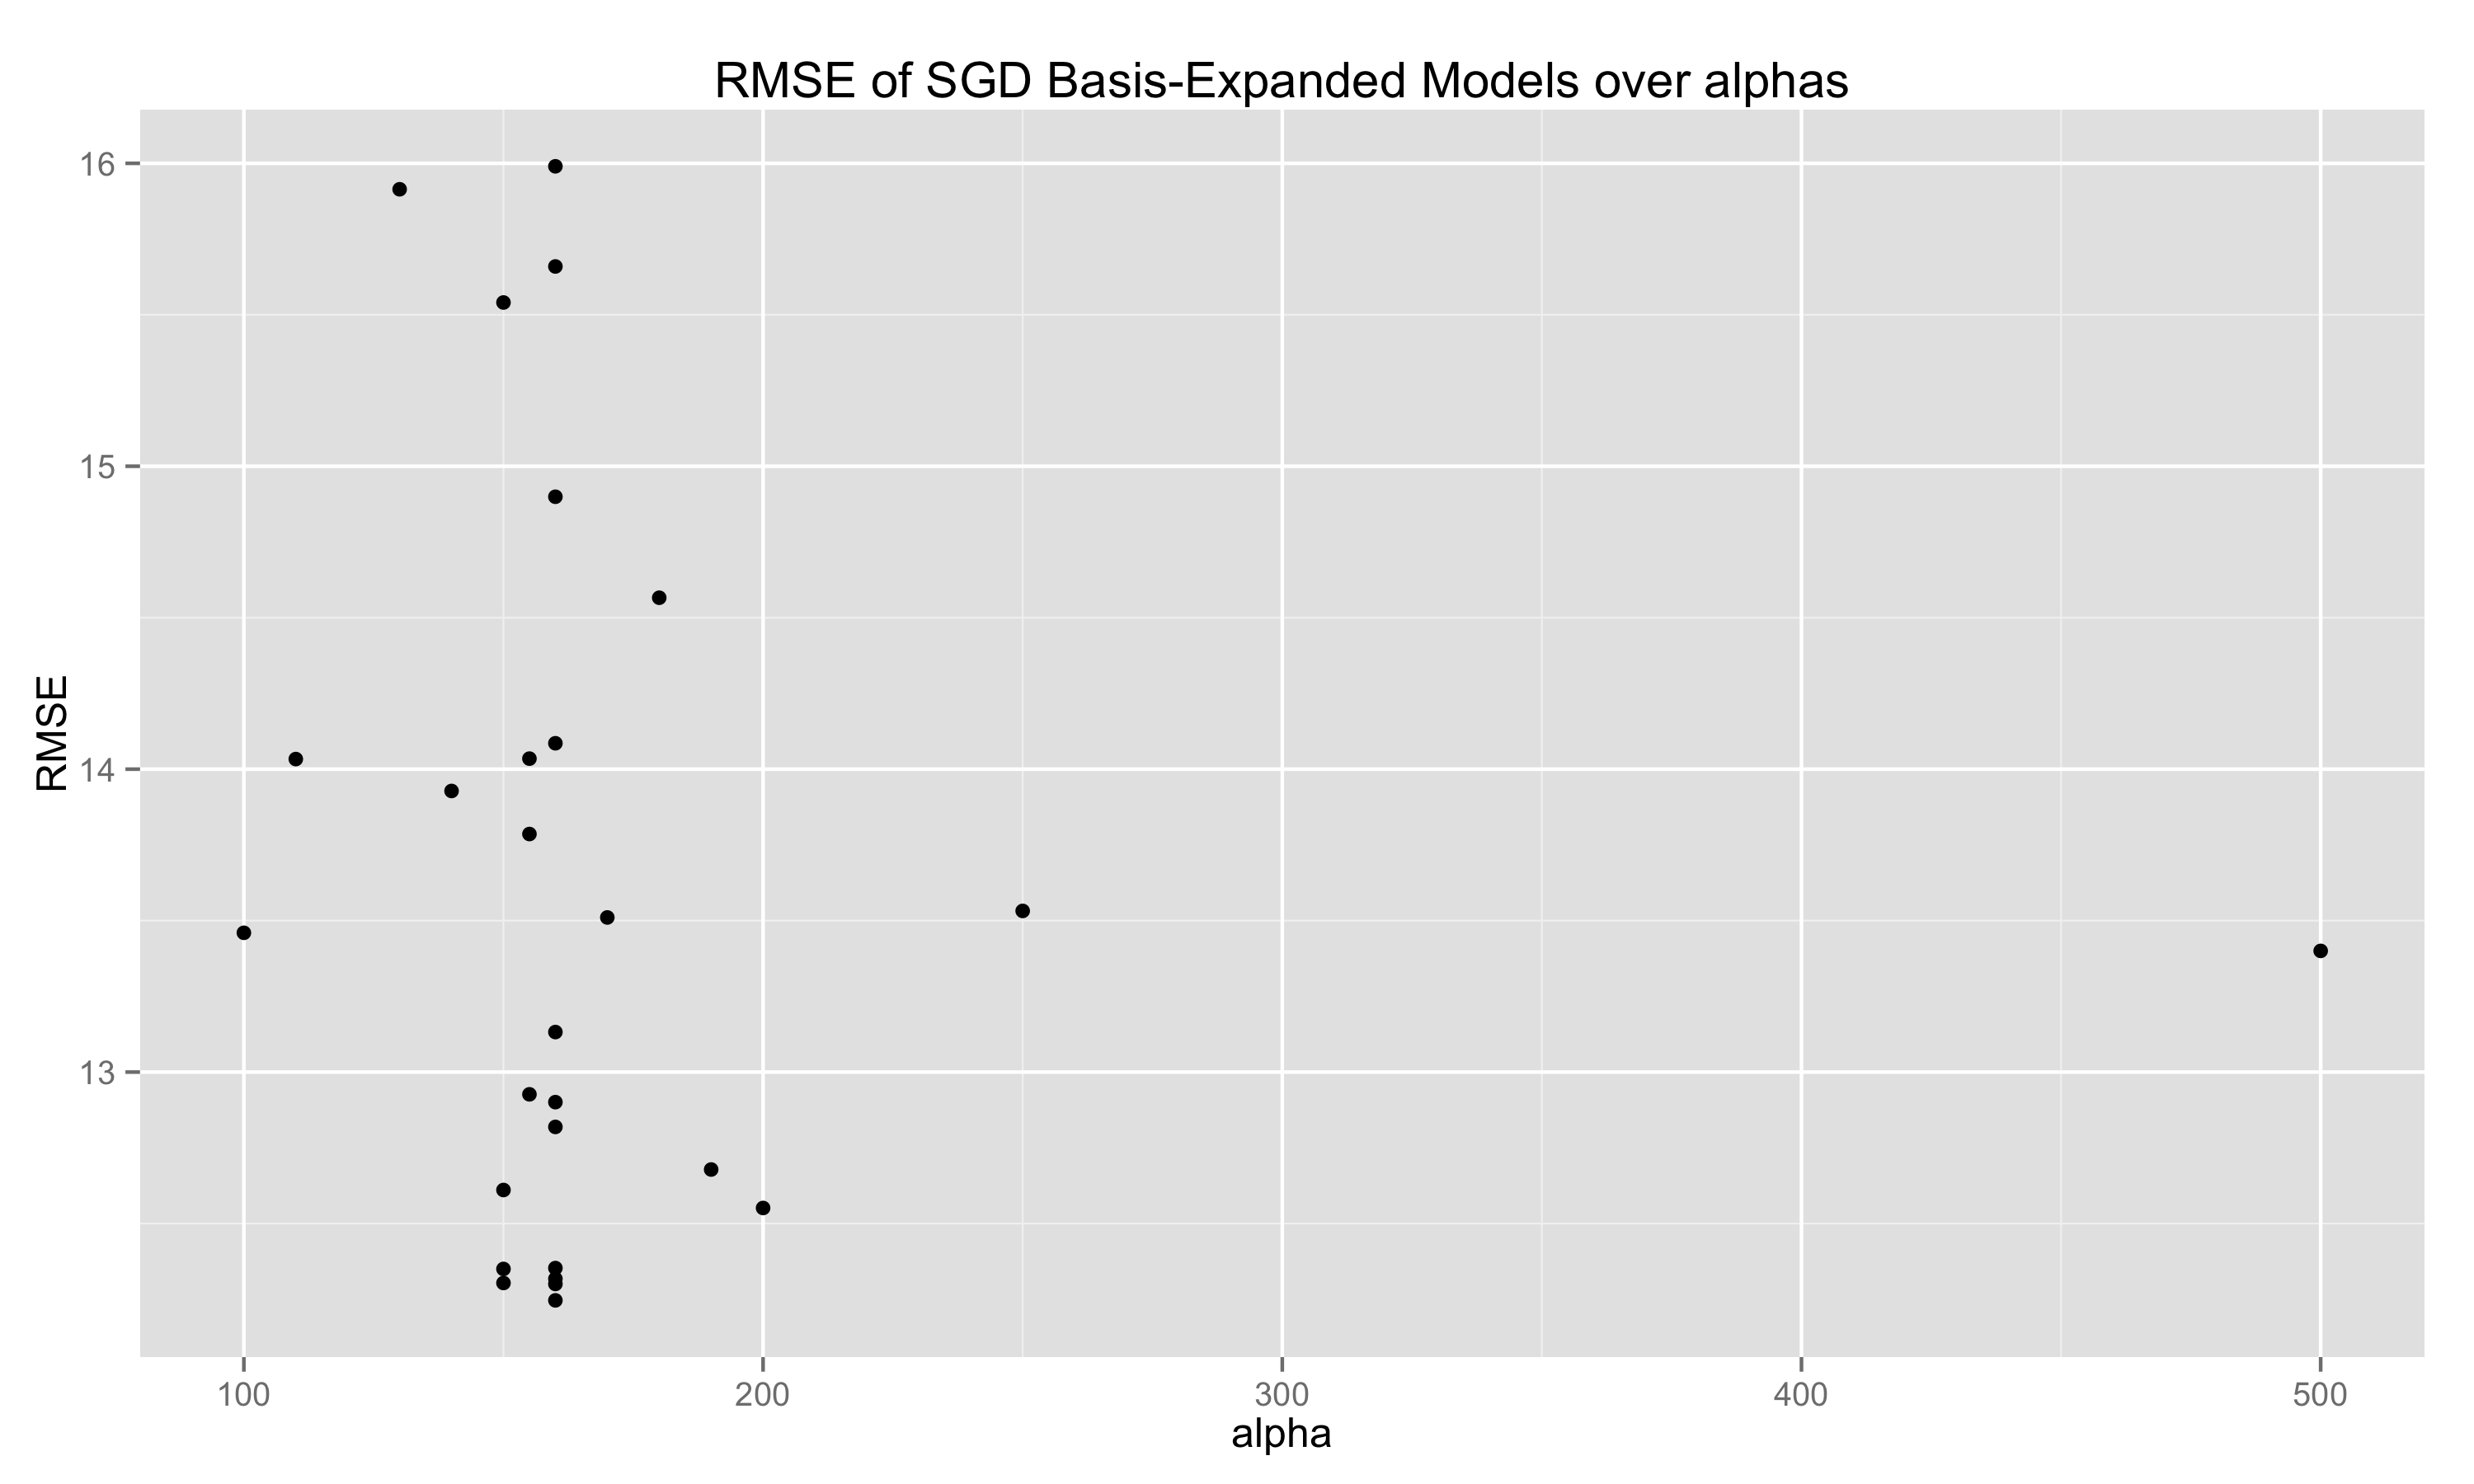
\includegraphics[width=155mm]{figs/basis_expand_RMSE_alpha.png}
\end{figure}
\subsubsection{MARS}
As described in Section \ref{sec:nonlinear}, we train a variety of MARS models, varying the \lstinline{fast_K} parameter.  We record training time and RMSE for each of the models.  As is clear from the following figure, the MARS models outperform both the simple linear SGD models and the non-linear basis-expanded SGD models significantly.  Even at the lowest values of \lstinline{fast_K}, where the training time is just under 5 hours, the RMSE is around 11.  At the highest value used, the RMSE drops all the way to just 9.91 (while training time is at a long, but not impossible 32 hours).  We see a convex shape in the RMSE over \lstinline{fast_K} plot, which indicates the likelihood that increasing \lstinline{fast_K} gives increasingly marginal decreases in RMSE, while the training time increases linearly.
\begin{figure}[H]
\centering
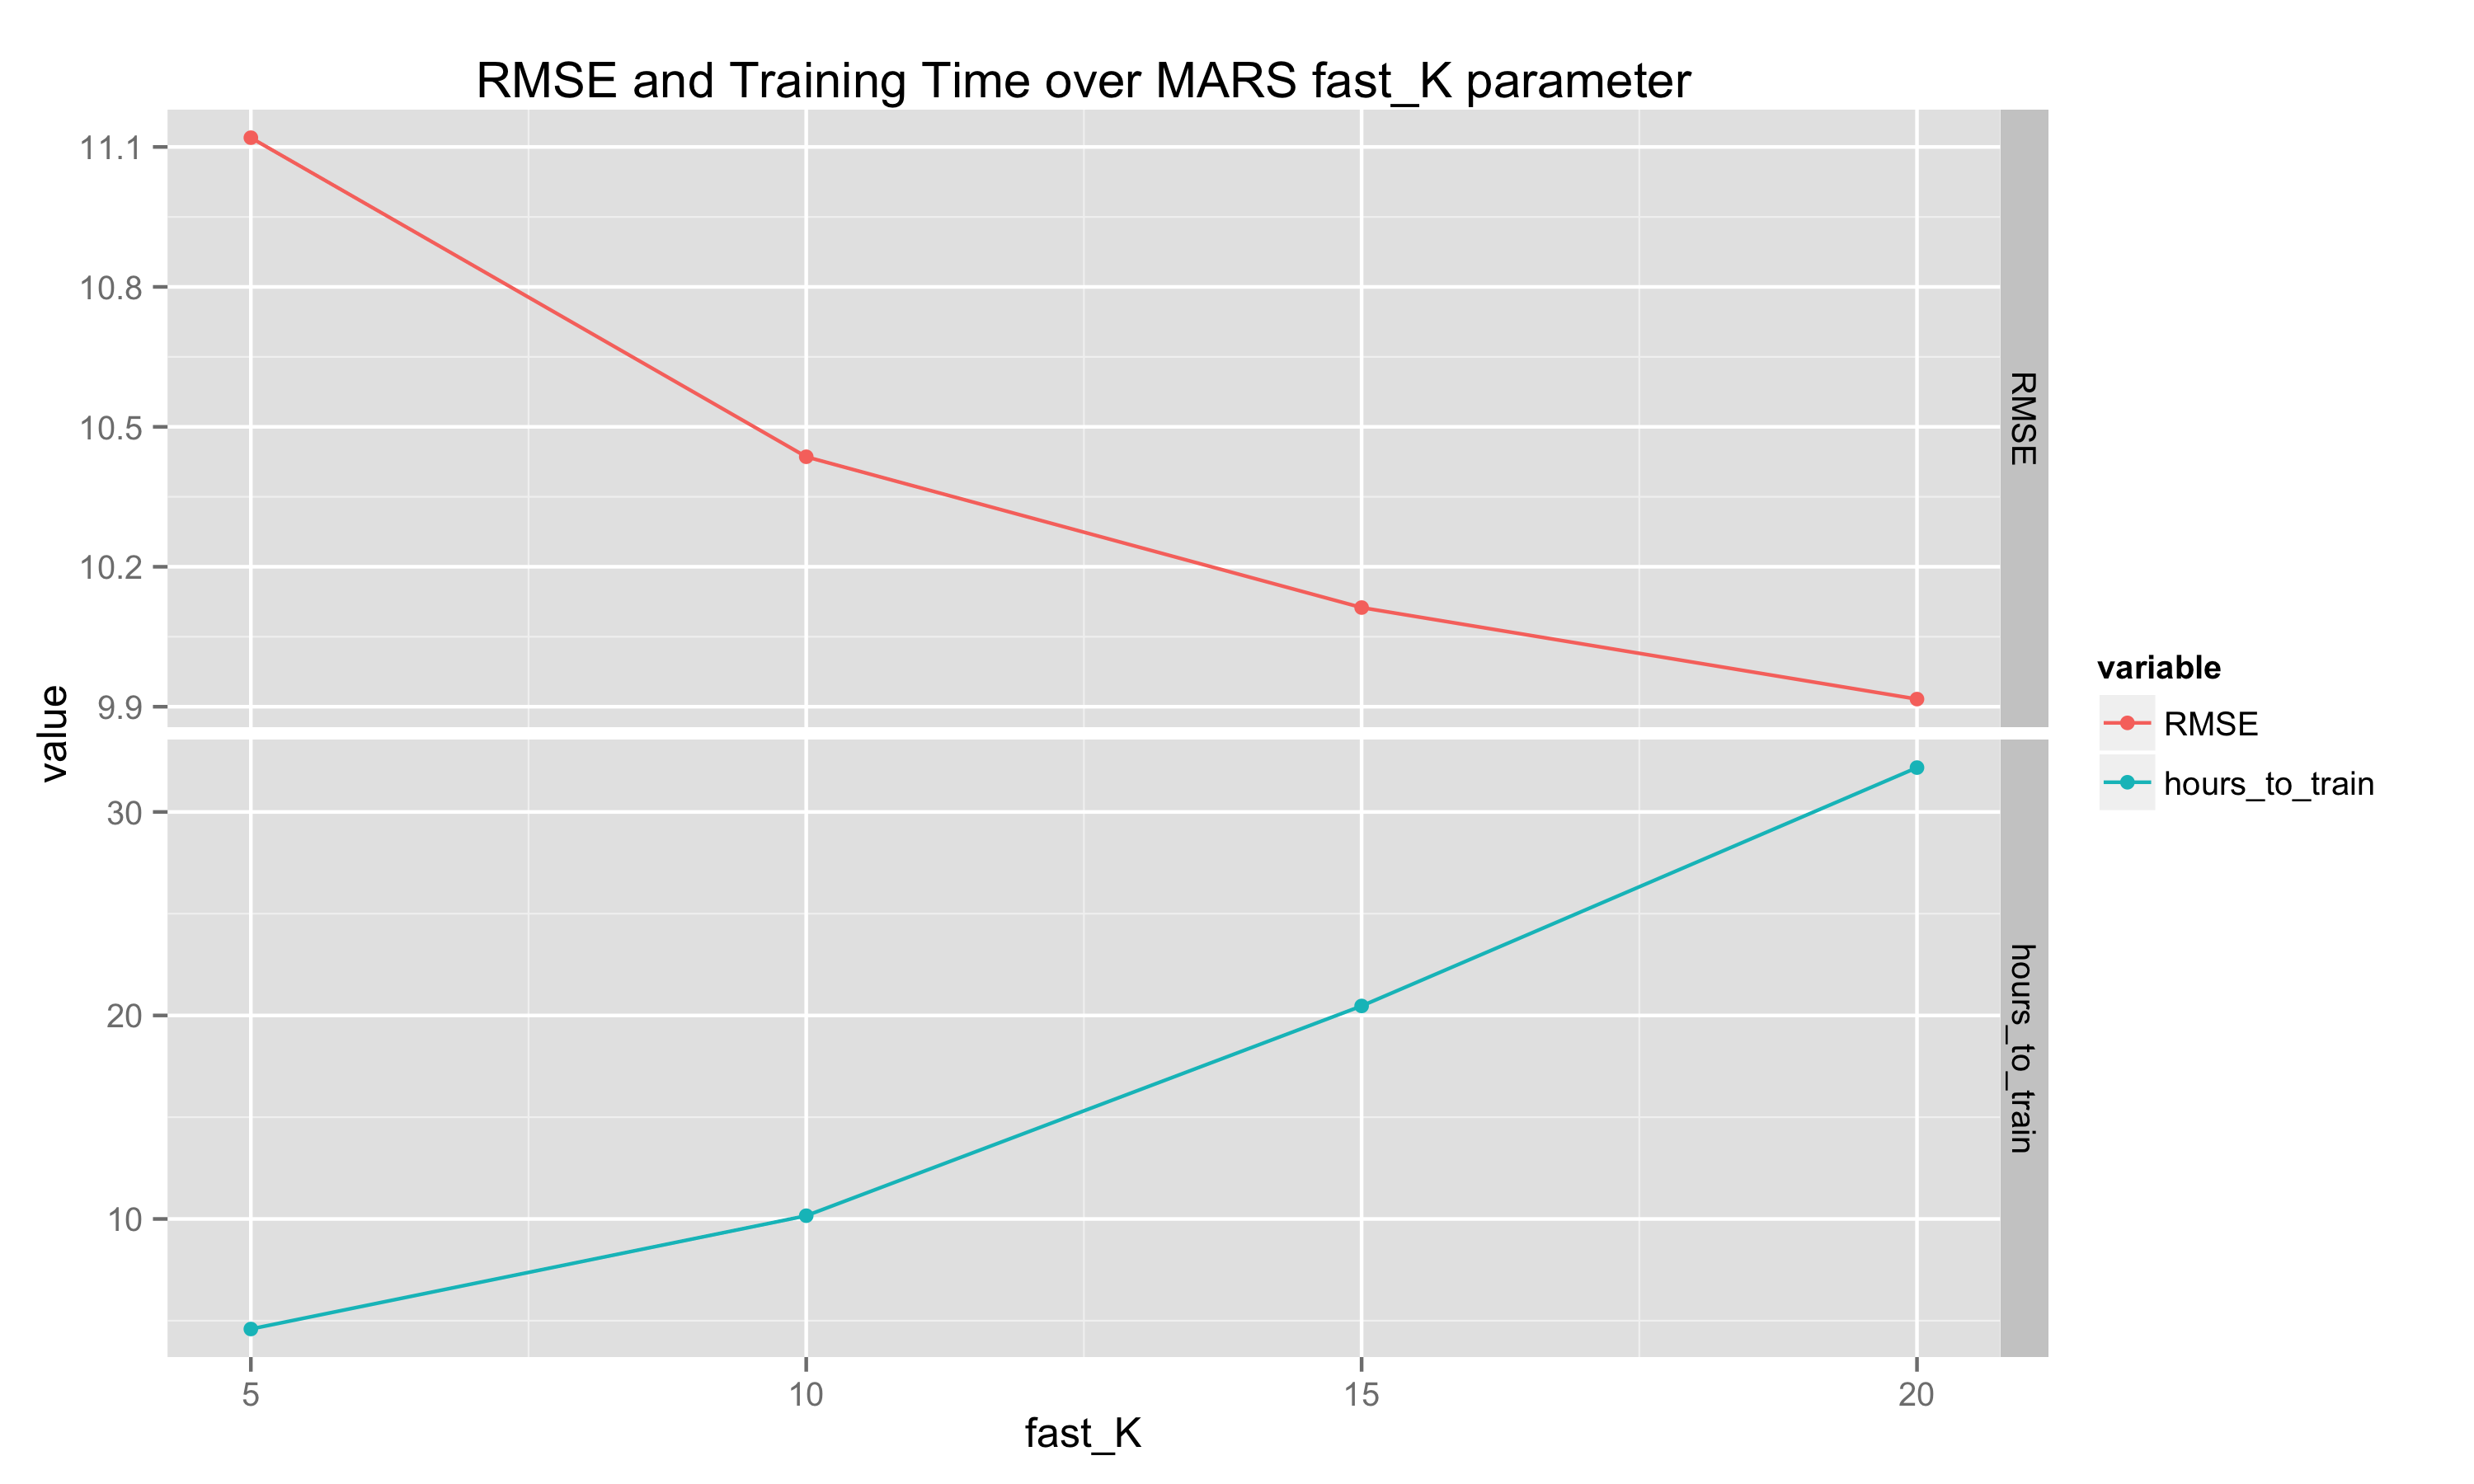
\includegraphics[width=155mm]{figs/mars_rmse.png}
% \caption{RMSE and training time of MARS models for various values of ``fast K''.}
\label{fig:mars_rmse}
\end{figure}
\section{Discussion}\label{sec:discussion}
Our original goal was to answer three questions, which largely relied on each other in succession.  First, for the problem of applying the direct perception paradigm for autonomous driving, we asked if immediately historical data is predictively useful.  We provided an unequivocally positive answer to this question by using ordinary least squares to fit simple and interpretable models for two models: Model 1, which used 500 convoluted image features for the current time step $t$, and Model 2, which used the 500 convoluted image features from the $t-1$ step alongside the current 500 features.  We saw that the distribution of the p-values for the coefficients corresponding to the $t-1$ features in Model 2 pointed to a very high significance level, one that completely confirms the importance of history.\par
Our second question, conditional upon a positive answer to the first, delved deeper -- we sought to rigorously determine not just if, but how much history was predictively relevant.  We answered this question by using stochastic gradient descent to fit a set of models that included incrementally more steps of history, and comparing the subsequent stacked information criterion metrics.  This process showed that for our TORCS data, including the most recent 7 data points gave the best performance with respect to the prediction validation set.\par
Finally, we simply wanted to validate that applying more complex, nonlinear models on data that included history would improve upon the predictive power of our linear recurrent models.  We fit both basis-expanded and MARS models, and found that the MARS models, which employ a similar iterative forward-backward training process to neural networks, achieved a performance significantly better than out linear recurrent models.\par
We were able to thoroughly answer all three of our questions with rigorous statistical analysis.  Note that we do not seek to compare our highest-performing nonlinear model to \cite{deepdriving} on a performance basis.  The goal for this paper was to establish confirmation of the importance and feasibility of using history and recurrency in the TORCS driving problem.  Therefore, a next extension of both this work the work of \cite{deepdriving} would make use of more advanced and powerful models as \cite{deepdriving} did, but also factor a recurrence in.  This could be done either through training a state-of-the-art non-recurrent model on recurrent data, similar to our methodology (for example, applying a convolutional neural network to recurrent data), or through using an actual recurrent model (a recurrent neural network, or more specifically, a Long Short-Term Memory neural network, applied to the non-recurrent data).
\newpage
\setlength{\bibsep}{1pt}
{
\bibliographystyle{ims}
\bibliography{RefDatBas}
}



\end{document} 
